%
% CS 321: Homework 1
%
% Due date: October 9, 2013
%
\documentclass[12pt]{article}

\usepackage{amsmath}
\usepackage{amssymb}
\usepackage{amsthm}

\usepackage{geometry}

%\usepackage{pgf}
\usepackage{tikz}
\usetikzlibrary{arrows,automata}
%\usepackage[latin1]{inputenc}

\title{CS321 - Homework 1}
\author{Trevor Bramwell}
\date{\today}

\begin{document}
\maketitle

\section*{Problems from 1.2}
\begin{description}
    \item[6] Let $L$ be any language on a non-empty alphabet. Show that $L$ and
          $\overline{L}$ cannot both be finite.

    \item
        \begin{proof}[Proof of $L$ and $\overline{L}$ cannot both be fininte]
            Let $L$ be any language on a non-empty alphabet. Assume $L =
            \overline{L}$ and both $L$ and $\overline{L}$ are finite.

            \ldots

            PROFIT
        \end{proof}

    \item[7] Are there languages for which $\overline{L^*} = (\overline{L})^*$?
\end{description}

\subsection*{Additional Problems}
For the additional problems, describe via an English sentence each of
the languages from the following Exercises in Section 1.2.

\begin{description}
    \item[14(b)] Let $\Sigma = \{a,b\}$. For each of the following
                 languages, find a grammar that generates it.

                 $L_2 = \{a^n b^{2n} : n \ge 0\}$.

    \item $L_2$ consists of two non-empty strings of $a$'s and $b$'s
        concatenated together, where the second string of $b$'s has
        twice as many symbols as the first string of $a$'s.
\end{description}

\begin{description}
    \item[15(a)] Find grammars for the following languages on $\Sigma = \{a\}$.

                 $L = \{w : |w|\, \mathrm{mod}\, 3 = 0\}.$
    \item $L$ consists of all strings - including the empty string
        - with lengths that are multiples of 3.
\end{description}

\begin{description}
    \item[18(b,d)]
        Using the notation from Example 1.13:
        \begin{eqnarray*}
          S \to& aA, \\
          A \to& bS,\\
          S \to& \lambda
        \end{eqnarray*}

        find grammars for the languages below. Assume $\Sigma = \{a,b\}$.

        (b) $L = \{w : n_a (w) = n_b (w) + 1\}$.

        (d) $L = \{w \in \{a, b\}^* : |n_a(w) - n_b(w)| = 1\}$.

    \item[(b)] Number $b$'s in the string is 1 more then the number of
        $a$'s.

    \item[(d)] The number of $a$'s and $b$'s in a string differ by 1.
\end{description}


\section*{Problems from 2.1}
\begin{description}
    \item[2(d)] For $\Sigma = \{a, b\}$. construct dfa's that accept the
                sets containing of all strings with at least one $a$ and
                exactly two $b$'s.

    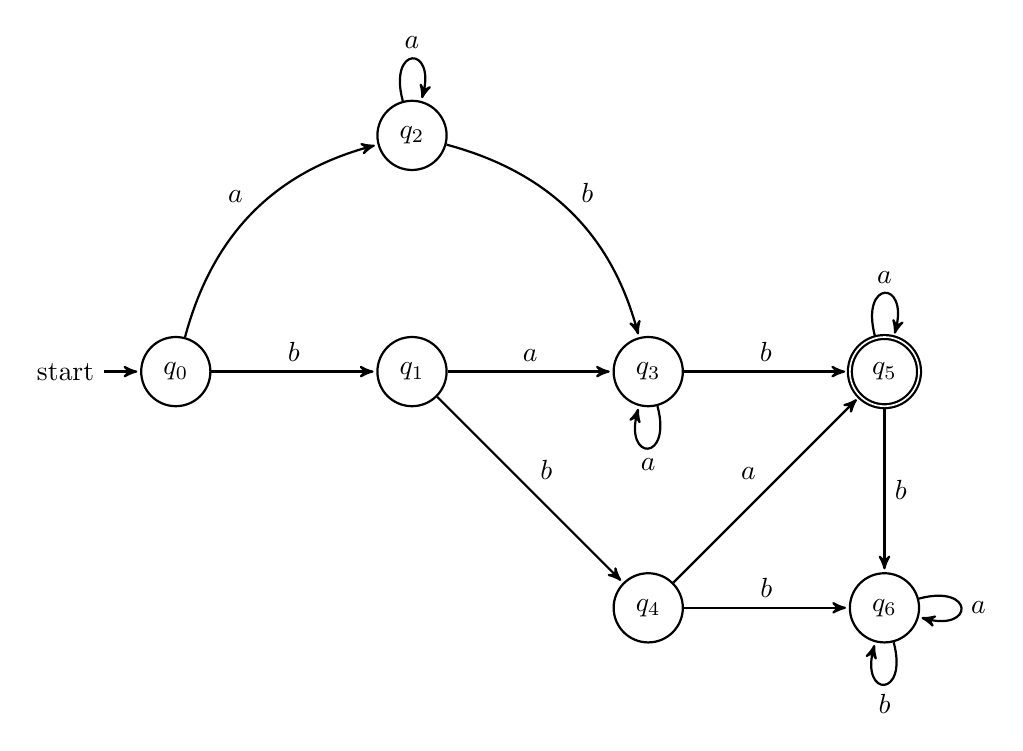
\begin{tikzpicture}[->,>=stealth',shorten >=1pt,auto,node distance=3cm,
                        thick]
      \tikzstyle{every state}=[fill=white]

      \node[state,initial]   (A)              {$q_0$};
      \node[state]           (B) [right of=A] {$q_1$};
      \node[state]           (C) [above of=B] {$q_2$};
      \node[state]           (D) [right of=B] {$q_3$};
      \node[state]           (E) [below of=D] {$q_4$};
      \node[state,accepting] (F) [right of=D] {$q_5$};
      \node[state]           (G) [below of=F] {$q_6$};

      \path (A) edge              node {$b$} (B)
                edge [bend left]  node {$a$} (C)
            (B) edge              node {$a$} (D)
                edge              node {$b$} (E)
            (C) edge [bend left]  node {$b$} (D)
                edge [loop above] node {$a$} (C)
            (D) edge [loop below] node {$a$} (D)
                edge              node {$b$} (F)
            (E) edge              node {$b$} (G)
                edge              node {$a$} (F)
            (F) edge [loop above] node {$a$} (F)
                edge              node {$b$} (G)
            (G) edge [loop right] node {$a$} (G)
                edge [loop below] node {$b$} (G);

    \end{tikzpicture}
\end{description}


\begin{description}
    \item[7(c)] Find dfa's for the following languages on $\Sigma = \{a, b\}$.

                $L = \{w : |w|\, \mathrm{mod}\, 3 > 1\}$.

    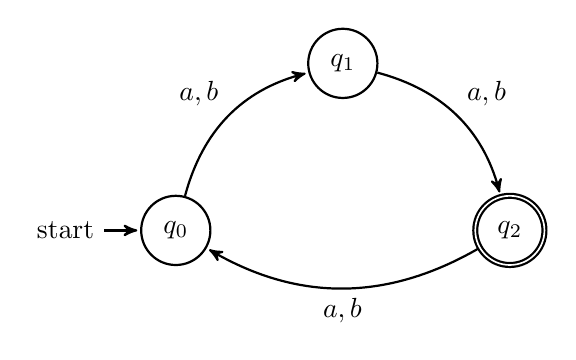
\begin{tikzpicture}[->,>=stealth',shorten >=1pt,auto,node distance=3cm,
                        thick]
      \tikzstyle{every state}=[fill=white]

      \node[initial,state]    (A)                    {$q_0$};
      \node[state]            (B) [above right of=A] {$q_1$};
      \node[state,accepting]  (C) [below right of=B] {$q_2$};

      \path (A) edge [bend left]  node {$a,b$} (B)
            (B) edge [bend left]  node {$a,b$} (C)
            (C) edge [bend left]  node {$a,b$} (A);

    \end{tikzpicture}
\end{description}

\begin{description}
    \item[9(c)] Consider the set of strings on $\{0, 1\}$ defined by the
                requirements below.  For each, construct an accepting dfa.

                The leftmost symbol differs from the rightmost one.

    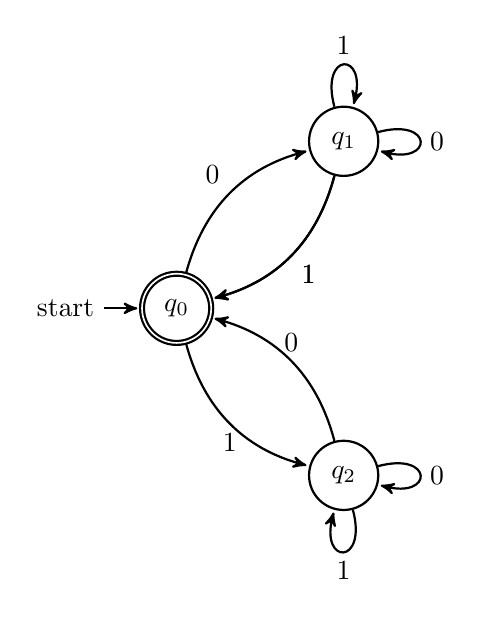
\begin{tikzpicture}[->,>=stealth',shorten >=1pt,auto,node distance=3cm,
                        thick]
      \tikzstyle{every state}=[fill=white]

      \node[initial,state,accepting]   (A)              {$q_0$};
      \node[state]           (B) [above right of=A] {$q_1$};
      \node[state]           (C) [below right of=A] {$q_2$};

      \path (A) edge [bend left]  node {0} (B)
                edge [bend right] node [below] {1} (C)
            (B) edge [loop above] node {1} (B)
                edge [loop right] node {0} (B)
                edge [bend left]  node {1} (A)
                edge [bend left]  node {1} (A)
            (C) edge [loop below] node {1} (C)
                edge [loop right] node {0} (C)
                edge [bend right] node [above] {0} (A);

    \end{tikzpicture}
\end{description}

\begin{description}
    \item[12] Show that $L = \{a^n : n \ge 4\}$ is regular.

    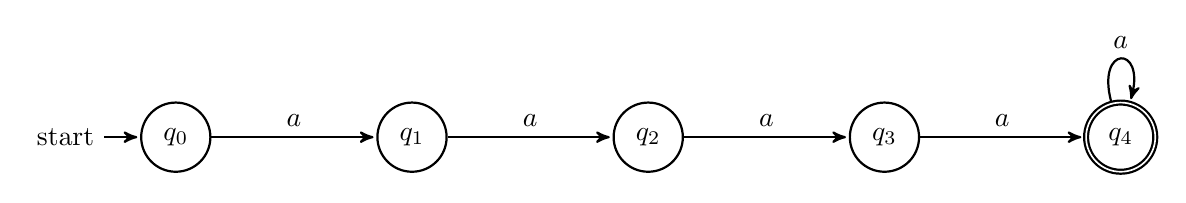
\begin{tikzpicture}[->,>=stealth',shorten >=1pt,auto,node distance=3cm,
                        thick]
      \tikzstyle{every state}=[fill=white]

      \node[state,initial]   (A)              {$q_0$};
      \node[state]           (B) [right of=A] {$q_1$};
      \node[state]           (C) [right of=B] {$q_2$};
      \node[state]           (D) [right of=C] {$q_3$};
      \node[state,accepting] (E) [right of=D] {$q_4$};

      \path (A) edge node {$a$} (B)
            (B) edge node {$a$} (C)
            (C) edge node {$a$} (D)
            (D) edge node {$a$} (E)
            (E) edge [loop above] node {$a$} (E);
    \end{tikzpicture}

    \item[17] Show that if $L$ is regular, so is $L - \{\lambda\}$.\\
              \emph{Hint}: We know that $L$ is regular. Thus there is a
              DFA $M$ such that $L = L(M)$. To solve this problem you
              need to describe how to form a new DFA $M'$ from $M$ such
              that $L(M') = L - \{\lambda\}$.  You can construct such an
              $M'$ by adding a single state to $M$ with the appropriate
              arcs. You need to provide an informal argument as to why
              your construction is correct.

\end{description}



\end{document}
